%\documentclass[3p,twocolumn]{article}
\documentclass[12pt]{article}

\usepackage{graphicx}
\usepackage{color}
\usepackage{url}
\usepackage{ifpdf}
\usepackage{hyperref}
\usepackage{xspace}

\setlength\parskip{-0.015em}
\setlength\parsep{-0.15em}

\newenvironment{shortlist}{
	\vspace*{-0.85em}
  \begin{itemize}
 \setlength{\itemsep}{-0.3em}
}{
  \end{itemize}
	\vspace*{-0.6em}
}

\usepackage{fullpage}
%\usepackage[top=tlength, bottom=blength, left=llength, right=rlength]{geometry} %http://en.wikibooks.org/wiki/LaTeX/Page_Layout
%\usepackage[margin=1in, paperwidth=5.5in, paperheight=8.5in]{geometry}

\usepackage{fancyhdr}
\setlength{\headheight}{16.0pt}
\pagestyle{fancy}
\headheight = 0pt
\headsep    = 25pt
\fancyhf{}
\fancyhead[OC]{\bf {\it \footnotesize{Jha et al: A Case for SAGA as an Access Layer for DCI}}}

\newif\ifdraft
% \drafttrue
\ifdraft
 \newcommand{\amnote}[1]{  {\textcolor{magenta} {***AM: #1}}}
 \newcommand{\jhanote}[1]{ {\textcolor{red}     {***SJ: #1}}}
 \newcommand{\olenote}[1]{ {\textcolor{blue}    {***OW: #1}}}
\else
 \newcommand{\amnote}[1]{}
 \newcommand{\jhanote}[1]{}
 \newcommand{\olenote}[1]{}
\fi

\newcommand{\dn}{\vspace*{0.33em}}
\newcommand{\dnn}{\vspace*{0.66em}}
\newcommand{\dnnn}{\vspace*{1em}}
\newcommand{\uppp}{\vspace*{-1em}}
\newcommand{\upp}{\vspace*{-0.66em}}
\newcommand{\up}{\vspace*{-0.33em}}
\newcommand{\shift}{\hspace*{1.00em}}

\newcommand{\T}[1]{\texttt{#1}}
\newcommand{\I}[1]{\textit{#1}}
\newcommand{\B}[1]{\textbf{#1}}
\newcommand{\BI}[1]{\B{\I{#1}}}
\newcommand{\F}[1]{\B{[FIXME: #1]}}
\newcommand{\TODO}[1]{\textcolor{red}{\B{TODO: #1}}}

\begin{document}

\title{Whitepaper: A Case for SAGA as Access Layer for Production
  Distributed Computing Infrastructures}

\author{Shantenu Jha$^{*1,2}$, Andre Merzky$^{1}$, Ole Weidner$^{1}$\\
  \small{\emph{$^{1}$Center for Computation \& Technology, Louisiana State University, USA}}\\
  \small{\emph{$^{2}$Department of Computer Science, Louisiana State University, USA}}\\
  \small{\emph{$^{*}$Contact Author \texttt{sjha@cct.lsu.edu}}}
  }


\maketitle

\section*{Aim and Audience of this White Paper}
The aim of this document is to inform providers, design architects and
users of production Distributed Computing infrastructures (DCI) of the
role and relevance of the SAGA API for their DCI. In particular, we
focus on how SAGA can increase the number of users and application
usage modes by providing SAGA as an access layer to DCI.

% It originally focused on Grid applications (i.e. applications running
% in Grid environments), but in fact maps well to all kinds of
% distributed infrastructures.



\section{Introduction}

SAGA is an acronym for "Simple API for Grid Applications". As the name
suggests, a simple API which facilitates the development and execution
of distributed applications on most types of distributed
infrastructure.  Modern distributed computing environments are very
complex infrastructures, and allowing applications to make use of
these complex systems is not trivial.  By defining a simple API, one
requires those complexities to be dealt with at levels other than
application code and development.  Simplicity of the interface is the
primary design principle and objective of SAGA.  Functional goals of
SAGA are:

\begin{enumerate}

\item Provide a stable programming interface to distributed
   application programmers and tool developers
 
\item Shield developer from heterogeneous and evolving
   infrastructures and middlewares

\item By providing the building blocks to distributed and remote
   operations enable the expression of high-level abstractions
   and support of distributed application requirements

\end{enumerate}

The fact that SAGA is an OGF standard ensures the community-wide
adoption and stability of the
API.  % SAGA's scope is defined top-down,
 % i.e. is determined by the high-level (i,e, application level)
 % requirements.
 % is the 80:20 rule: 80\% of functionality at 20\% of the complexity.

\section{The SAGA Landscape}

 \subsection{SAGA API Specification}

  The SAGA API specification is object oriented, and language
  independent (the API is defined in IDL).  The API is structured into
  various packages (e.g. jobs, replicas, streams, etc.).  Those
  packages have limited dependencies amongst each other - not all SAGA
  implementations implement all packages.  All API packages share
  certain properties: how are synchronous methods expressed, how are
  notifications realized, how are security tokens expressed, what
  types of exceptions are defined, etc.  Those properties are
  specified in the SAGA-Core, the API's look and feel.

  That design of the SAGA API allows to specify additional API
  packages, which adhere to the same look-and-feel.  In fact, several
  such API packages have already been defined (e.g., Service
  Discovery, Remote Procedure Calls etc.), and are standardized as
  well, or are in the process of being standardized.

 \subsection{SAGA: A Community Specification}

  The SAGA API specification has been developed and guided by the
  broader distributed computing community at the OGF.
  (\url{http://www.ogf.org/}).  An analysis of the requirements led to
  abstractions that were mapped into different SAGA API packages,
  while ensuring that (a) the overall usability (e.g. the API
  look-and-feel) was consistent over the whole scope of the API, (b)
  the API functionality maps relatively well onto existing middleware
  features, and (c) the API is simple to use.  The API is simple, even
  if the semantic translation and across layers and maintaining
  implementation fidelity for middleware specific features is not
  trivial.

  The SAGA standardization effort is closely syncronized with other
  specification and community efforts, within and outside of OGF.  In
  particular, OGF groups ensure that SAGA semantics map well to lover
  level specifications, such as JSDL, BES, GridFTP, etc.   But also, 
  and possibly more importantly, it is now widely and independenly
  acknowledged that a uniform, simple and stable access layer is
  neccessary (but not sufficient) to improve end user experience on
  distributed computing infrastructures, and that SAGA can indeed play
  that role for a specific set of use cases.  As such, SAGA is now
  integral part of the GIN (Grid Interoperation Now) community effort,
  and also plays an active role in current efforts like OGF's PGI
  group and US's XD proposals.
  
  % The SAGA Working group within OGFs
  % application area first collected a set of ca. 20 use cases,
  % considered representative for a wide range of distributed scientific
  % applications. Based on these use cases, the group defined a set if
  % high level abstractions commonly required by those use cases.
  
  % The fact that the resulting SAGA API specification is a rather hefty
  % document is not a token of the complexity of the resulting API, but
  % rather a token for the level of detail the API semantics is specified.
  % Also, it must be noted while the resulting API is indeed rather simple
  % to use, it is, to most parts, rather difficult to {\bf implement} -
  % ease of implementation has {\it not} been a design goal for SAGA.
  
  % on a different layer,
  % i.e. within the SAGA API implementation. This is on purpose, as it
  % allows to keep those complexities out of the application code, which
  % is a declared goal of SAGA.

  \jhanote{SJ to shorten a bit..}


 \subsection{SAGA Components}

  As discussed, the SAGA API specification is language independent.
  The SAGA distributions contain various language \I{bindings} for
  that API.  The SAGA-Core distributions deliver those bindings as
  class  files for Java, as modules for Python, and as shared and/or
  static libraries for C++.

  SAGA as an API would be rather useless if it would not also offer
  bindings to the various middlewares.  Those bindings are, for all
  major SAGA implementations, provided as \I{adaptors}.  Some simple
  adaptors are usually packaged with the SAGA-Core distributions, but
  otherwise are packaged and distriubuted separately (details see in
  section~\ref{ssec:adaptors}).

  While SAGA is foremost an API, the SAGA distributions support end
  users in a variety of ways.  In particular, the SAGA distributions
  also include command line tools implemented via the SAGA API, and
  higher level libraries for common distributed programming patterns,
  also basing on the SAGA API.  Further, the SAGA distributions
  provides comprehensive support to compile, link and run SAGA
  applications (configure scripts, make support, runtime wrappers,
  developer tutorials , etc).

  Command line tools are, in our experience, amongst the first
  components of any distributed middleware to be exploited by end
  users.  SAGA-C++ provides a set of command line tools which
  basically cover the complete semantic set of SAGA API calls, such as
  job submission and management, file management, replica management,
  etc.

  Several SAGA based projects are actively developing and using higher
  level programming abstractions, such as pilotjobs, bigjobs,
  mapreduce, or workflows.  Such components are routinely installed
  and used by a number of user communities, and represent significant
  added avlue, although they are not part of the SAGA core code base.
  It should be noted that the SAGA Python bindings, which are usually
  installed by default, are very frequently used to provide tooling and
  higher level programming abstractions.


 \subsection{SAGA Core: Implementations and Deployment}

  \subsubsection{SAGA Implementations}

   The language independent SAGA API specification has been mapped to
   multiple programming languages, in particular to C++, Java and
   Python.  Multiple implementations exists, the most notable ones are
   SAGA-C++, JSAGA and JavaSAGA.

   SAGA-C++ is, as the name suggests, a C++ implementation of the SAGA
   API, mainained by CCT/LSU, and a growing international community.
   The SAGA-C++ development is in close lockstep with the API
   specificatin efforts, and the most widely used SAGA implementation
   to date. 
   
   JSAGA (from IN2P3 in France) and JavaSAGA (from the Vrije
   Universiteit, Amsterdam) are API compatible Java implementations
   (they use the same set of abstract class definitions).  JSAGA
   caters to an active, but small user community in France, and
   supports a realitvely large set of adaptors for the job and file
   API packages.  JavaSAGA is mostly a academic research vehicle,
   which bases its middleware bindings mostly on JavaGAT (its
   predecessor), and sees some uptake in the Netherlands and the
   German D-Grid project.

   All three implementations provide python bindings - the Java
   implementations realize those via Jython, the C++-implementation
   via Boost-Python.  The two Python bindings are at the moment being
   unified, and have already been shown to be interoperable.  The
   Python bindings are implemented as a wrappers around the C++ and
   Java implementations, and are thus able to utilize their complete
   set of middleware adaptors.

   This white paper focuses, from here on, on the SAGA-C++
   implementation.


  \subsubsection{Important SAGA Deployments}

   The different SAGA implementations, and in particular SAGA-C++,
   have by now been in use in different user communities for a number
   of years, and thus have matured enough to enter the field of
   production cyber infrastructures.  At the same time, the number of
   supported backends has grown to a level that basically all current
   production infrastructures are supported (e.g. for jobs we support
   ARC, gLite, Globus, Condor, PBS, Torque, DRMAA, EC2, Eucalyptus,
   BES, Naregi, Unicore, SMOA, Genesis-II, fork, and
   ssh)\footnote{\url{http://cyder.cct.lsu.edu/saga-interop/mandelbrot/demo/today/last/}}.

   SAGA has so far been successfully and routinely used on the
   TeraGrid, LONI, FutureGrid, DEISA, NAREGI/RENEKI and a number of
   smaller, more localized DCI. It has also been used by a range of
   e-Science projects such as EGEE, DGrid, VPH etc.

   SAGA-C++ has one major external dependency, which is
   Boost\footnote{\url{http://www.boost.org/}}, a set of C++ headers
   and lbraries widely used in the C++ community.  While Boost itself
   is a fairly complex code base, it is routinely packaged by the
   various Unix distributions, and thus usually available out of the
   box.  Further, SAGA-C++ is able to compile against a wide range of
   Boost releases, including those which are the default versions for
   the currently used Linux distributions.  Postgresql client
   libraries are not strictly required, but recommended for some of
   the core SAGA functionality.

   While SAGA is relatively easy to deploy in applications space (i.e.
   user space), its overall goal of improving the end user experience
   of distributed systems benefits greatly from system level
   installations.  It is straight forward to install SAGA in user
   space (\T{configure; make; make install}), but in our experience,
   the correct environment setup to use a SAGA installation in user
   space is still a stumbling stone for many end users
   (\T{LD\_LIBRARY\_PATH} etc).  We thus prefer SAGA to be available
   in system space, which lowers the entry barrier significantly.  

   We are currently working to provide binary releases, in the form of
   Debian and Ubuntu packages, and RPMs.  Also, we are currently
   integrating SAGA into NMI and ETICS build and testing environments,
   which we hope will lower the effort for system level installations
   significantly.


 \subsection{SAGA Adaptors Implementations}
 \label{ssec:adaptors}

  Interestingly, all three SAGA implementations discussed above are
  adaptor based: a relatively small library provides the SAGA API, and
  a set of adaptors translate the SAGA API calls into the respective
  middleware operations.  It is those adaptors which encapsulate most
  of the complexity which was formerly present in the applications
  layer.  While SAGA adaptors are relatively easy to implement (or at
  least as a prototype), they require significant maintainance effort
  to keep up with the middleware intricacies and evolution.

  SAGA-C++ supports the implementation of adaptors with a tool, which
  generates a complete, but semantically empty adaptor stub.  The
  adaptor developer has then to fill that stub with the respective
  native middleware calls.  SAGA-C++ further provides tools and
  support for adaptor compilation, documentation and packaging.

  For a list of adaptors that are currently supported by SAGA-C++,
  refer to: \url{http://saga.cct.lsu.edu/software/cpp}.



\section{SAGA Usage and Active Projects}

 \subsection{SAGA usage modes}

  Although SAGA is foremost an API, the SAGA distributions support end
  users in a variety of ways.  In particular, the SAGA distributions
  also include command line tools implemented via the SAGA API, and
  higher level libraries for common distributed programming patterns,
  also basing on the SAGA API.

\subsection{SAGA Active Projects}

 \subsubsection{Standards promote Interoperability}

 \subsubsection*{ExTENCI}
 \url{https://sites.google.com/site/extenci/} ExTENCI is an NSF funded
 2 year project to promote interoperability between the TeraGrid
 (and/or its successor -- XD) with the OSG (and its successor).
 The role of SAGA is provide a common job-submission mechanism
 across TeraGrid and OSG, for both command-line access as well
 as for Cactus based application via Gateway.
 The different application scenarios that are/will be supported are:
 \begin{itemize}
 \item Ensemble of Cactus Simulations (NumRel, EnKF (Petroleum Eng))
 \item Multiphysics Code (GR-MHD, CFD-MD)
 \item Spawning Simulations (Realtime ‘outsourcing’ from
   BlueWaters/Ranger to specialised architectures or less powerful
   resources)
 \end{itemize}


\subsubsection*{VPH - Efficient Free Energy Calculation Methods using
  HPC Interoperation}

The Virtual Physiological Human (VPH) project is concerned about
providing computer models for personalized patient specific healthcare
and also trying to create tools for modelling and simulation of human
physiology. There are multiple use cases: The first consists of
simulations of so-called “ensembles” which are non-interactive and
thus their computation can be considered embarrassingly parallel. The
second step consists of loose coupling of the simulated ensembles,
which requires limited interaction between the jobs.

This is a computationally intensive problem and could utilize as many
HPC resources as could be possibly made available or acquired. Current
efforts are aimed at using the high-end TG and DEISA (soon to be
PRACE) machines collectively to finish a work-load. The underlying
kernel is the same (NAMD) but the execution management is needs
to be intereoperable; this is provided by SAGA.

\subsubsection*{gLite / Ganga} 

GANGA is a very commonly used tool to submit jobs to EGI/EGEE. GANGA
does not provide explicit support for submission to globus-based
systems. There exist multiple application (eg LatticeQCD) that would
benefit from both HPC-HTC job submission capabilities. Therefore Ganga
uses SAGA and its globus adaptor to extend the capabilities of GANGA.
See
\url{http://svnweb.cern.ch/world/wsvn/ganga/trunk/ganga/python/GangaSAGA/Lib/SAGA/#path_trunk_ganga_python_GangaSAGA_Lib_SAGA}

\subsubsection*{RENKEI/NAREGI}

The RENKEI e-Science project is using SAGA in two distinct ways: as
shown in Fig.~\ref{fig:renkei}, one mode is as an access layer to
multiple middleware distributions, including but not limited to globus
and Naregi.
\begin{figure}[t]
      \centering
      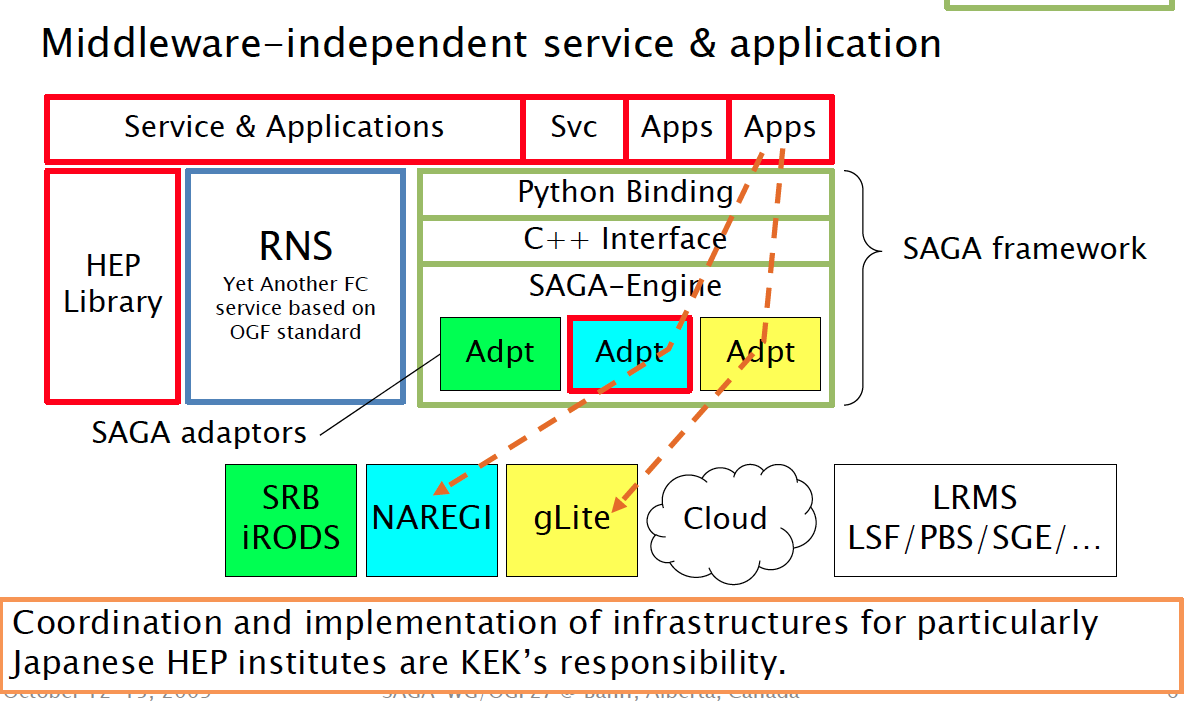
\includegraphics[width=0.6\textwidth]{saga-renkei.png}
      \caption{\footnotesize }
      \label{fig:renkei}
\end{figure}
The second is to provide Python scripting capabilities for simple
workflows executing over multiple resources -- job submission, task
management (coordinated execution) and data/file management.  See
details at the following:
\url{http://saga.cct.lsu.edu/projects/tools-and-infrastructure/kek-1}





\subsubsection{Applications Scenarios}

\subsubsection*{FEDEX: A SAGA-based Runtime Framework for Dynamic
  Execution of Multi-Physics Simulations}
SAGA provides a runtime framework for dynamic execution (FeDEX) which
can be used to support the execution of coupled multi-physics
simulations. This is being used by several projects including the \$2M
NSF-funded Cybertools Project (\url{http://www.cybertools.org}) and
the EU FP7 Mapper Project (\url{http://www.mapper-project.eu/}).

\subsubsection*{NeuGrid / UWE}
Use SAGA based Glueing Service and DAG-execution for Medical Imaging
and workflow on the EGI/EGEE.  See following:
\url{http://www.futuremedicine.com/doi/full/10.2217/fnl.09.53} \&
\url{http://www.neugrid.eu/download/deliverables/D6.2_final.pdf}

\subsubsection{Tooling}
``One persons application is another persons application''. So what
distinguishes a tool from an application?  In our viewpoint, a couple
of items: The end-user is also the developer of an application;
typically these are different for a tool. Additionally, typically
there is a single user of an application, whereas by definition there
are multiple users of a tool. Both these attributes hold for the tools
discussed below.

% \subsubsection*{JSAGA}

\subsubsection*{EGI- Service Discovery}

The SAGA Information System Navigator API provides a uniform interface
to access additional details published by the information system.  For
details see \url{http://hepunx.rl.ac.uk/egee/sa3-uk/sd/} and
\url{http://rgma03.pp.rl.ac.uk/InfoBrowser/}

\subsubsection*{SAGA-based Pilot Jobs (BigJobs)}

Pilot-Jobs provide a very common usage model for distributed computing
infrastructure. There exist many/multiple pilot-job implementations
for different DCI, often with there own semantics but definitely with
their own access/usage APIs. SAGA provides a common API to access {\it
  different} Pilot-Jobs; this API is called the BigJob API. A BigJob
provides a concrete implementation of the API along with specific
adaptor so as to be usable for a given backend. See
Fig~\ref{fig:sagabigjob} for an example of this well-defined API and
its usage on four different infrastructure types.
\begin{figure}[t]
      \centering
      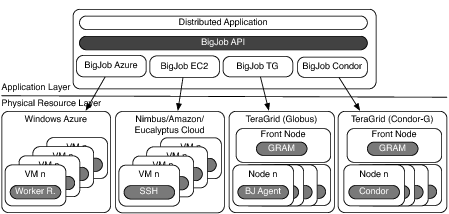
\includegraphics[width=0.6\textwidth]{distributed_pilot_job.png}
      \caption{\footnotesize }
      \label{fig:sagabigjob}
\end{figure}

The BigJob API provides an interesting example of a ``higher-level
abstraction'' that build-upon the {\it primary} distributed computing
functionality that SAGA provides. Another example of such a
higher-level abstraction is a DAG executor (called diggedag) that uses
the same job-model as SAGA along with other consistent semantics.

\subsubsection*{Computational Biology Gateways}

Gateways have emerged as a successful resource access and job
submission environment.  In particular, where a community of users
have similar usage requirements and patterns, Gateways are particular
effective.  SAGA has been used to build and design Gateways in such a
way that they are agnostic to the details of the underlying DCI. For
two examples see, DARE-RFOLD (\url{http://cyd01.cct.lsu.edu/}) and
GridChem (\url{http://www.gridchem.org}).  SAGA provides a critical
risk mitigation strategy via the the standards based approach that it
supports.

\section{Analysis of Use Cases}

Distributed Computing is more than just submitting isolated jobs.  It
is also about federating resources dynamically; about coordinated
execution of heteregeneous and dynamic workloads; it is about
distributed data management etc. So while SAGA is used for multiple reasons. Three primary usage modes of SAGA
are the following: (i) Simplifying access layer, (ii) building block
for tools and distributed execution execution, and (iii) a distributed
scripting and programming capability.


\jhanote{This should move: A primary objective of SAGA is to support
  and simplify the implementation of distributed applications.  As
  described earlier, that is achieved by providing a library which
  implements the SAGA API.}

% However, distributed applications have to {\it wrestle} with
% distributed infrastructures at more layers than just APIs, and the
% SAGA distribution tries to address a number of additional issues as
% well. In particular prototyping, deployment, and application
% enrollment and bootstrapping are continous concerns for end users.

\subsubsection*{Providing Distributed Scipting and Programming Capbility}
The Structural Biology Grid (\url{http://SBGrid.org}) currently
implements sophisticated analysis and user-defined pipelines. However,
these are inherently localized and confined to specific
infrastructure.  Replacing ``local python'' calls with ``distributed
(SAGA) python'' calls would enable the seamless utilization of
DCI. This provides a simple mode of extensibililty of infrastructure,
without any major refactoring of code. The advantages of this to the
end-user is obvious; the lowered barrier-to-entry for novel users and
communities will increase the ease and uptake of DCI thus benefitting
DCI providers/organizations.  As part of the ExTENCI project, SAGA
will make major advances towards becoming a broadly usable
programmatic access layer to Condor/OSG.

\subsubsection*{Application Prototyping and Tooling}

The SAGA Python bindings have been proven to be immensely helpful for
application prototyping.  But also, they are very helpful when
interactively testing remote operations (in the interactive Python
interpreter / Python shell).  Finally, it is very easy to implement
small command line tools in Python, which are able to mimic and test
smaller portions of the overall application.  For example, it is
straight forward to implement a specific job control component of an
application in a stand alone Python script, and to later include the
same functionality in the application proper, with the confidence that
the semantics of the remote operations will be well
preserved. %(remember: the SAGA specification is very strict about
   %the definition of semantics).

\subsubsection*{Application Development}

%    According to the SAGA use case analysis\cite{saga-uc}, and to our
%    own experience in developing distributed applications, the set of
%    funtionality required for such applications is rather limited.
%    However, as that functionality is provided in very different ways,
%    by the various distributed middlewares available today, application
%    complexity has historically increased significantly for any single
%    remote operation used by the application.

  The SAGA API provides very concise and high level method calls which
  cover the vaste majority of distributed operations, as required by
  the target user community -- scientific application and tool
  developers.  Further, as the API specification and implementation is
  \I{standardized}, and thus stable, it allows for a 'write once, run
  anywhere' approach, which is in general not available otherwise (or
  at least not without \I{significantly} increase of application
  complexity).

% \subsubsection*{Application Deployment}

% \subsubsection*{Runtime Configuration}

   
\section{Relevance to EGI/UMD}

EGI (and EMI) encompass, at the moment, the three major European
middlewares: Unicore, ARC and gLite.  Additionally to the respective
native service interfaces and client access layers, EMI is in the
process of defining a unified service interface for these systems.
EGI users have thus be able to handle the three existing interfaces,
and have to be able to cope with the evolution of the new EMI
interface, \I{or} have to limit their selection of available resources
(by selecting resources which support their preferred access layer),
\I{or} they can be shielded from the middleware heterogeneity and
evolution by an intermediate layer (tooling and/or API).
 
SAGA is one way to provide that additional, shielding abstraction
layer, and should thus, in our humble and biased opinion, considered
as a candidate for inclusion into UMD.  Additionally we argue that
SAGA is \I{easier} to use than the native APIs, as it provides higher
levels of abstractions.  Further, SAGA has shown well to work with
other infrastructures, in particular with Globus, which IGE will
additionally provide to UMD (In fact first few success stories of IGE
are built around applications that use SAGA.).  Those points hold for
both programmatic access via the SAGA API, as for the scripting
(Python) and tooling (command line) components provided by the SAGA
distribution.

Support of SAGA for the UMD/EGI user base also provides the additional
benefit to the end user that applications codes and runtime
environments are compatible, and in fact interoperable, with OSG
(Extenci project), TeraGrid/XD, LONI, and other distributed
cyberinfrastructures.

The "EGI-InSPIRE UMD Roadmap" (EU deliverable D5.1) lists the
capabilities planned to be provided by UMD.  SAGA does actually not
map into any single of those capabilities, but is rather cross-cutting
over most of them: it either provides explicit access, or implicit
coverage, for 14 out of 21 capabilities.  At the same time, SAGA does
not really \I{provide} any of those capabilities, as it is not a
middleware service, but 'just' an API.  While 'access' and
'interfaces' are mentioned as general project objectives (see Section
VII on page 3), the document actually misses an explicit capability
covering the client side access to EGI resources and middleware
capabilities.  The assumption is likely that this comes separately
with each capability, but we would like to remind that the sum of
those access components will not neccessarily form a coherent,
consistent and simple interface for the end users (it might, of
course, depending on the specific capability providers, but the UMD
document is at the moment not evaluating that aspect).

On the other hand, the "EGI-InSPIRE Standards Roadmap" (EU deliverable
D2.5) lists standardized a Client API as one of the functional
capabilities supporting interoperability.  SAGA is mentioned
explictely as one possible approach for that (page 18, Section
3.2.25).

The "EMI Technical Development Plan" (DNA 1.3.1) includes specific
parts of SAGA (service discovery and information system navigation) as
components (page 15), and further lists SAGA (in general) as one of
its "further objectives" (page 25).  The SAGA community is, as we
discussed above, actively participating in the GIN and PGI efforts,
with the explicit goal to ensure that future PGI and EMI interfaces
map well to the abstractions provided at SAGA level.


\subsection{SAGA as a Standardized Programmatic and Access Layer:
  Advantage to DCI Providers}


% As part of the ExTENCI project, SAGA will make major advances towards
% becoming a broadly usable programmatic access layer to Condor/OSG.
% For example the Structural Biology Grid that currently
% (\url{http://SBGrid.org}) currently implements sophisticated analysis
% and user-defined pipelines. However, these are inherently localized
% and confined to specific infrastructure.  Replacing ``local Python''
% calls with ``distributed (SAGA) Python'' calls enables the seamless
% utilization of DCI. This provides a simple mode of extensibililty of
% infrastructure, without any major refactoring of code. The advantages
% of this to the end-user is obvious; the lowered barrier-to-entry for
% novel users and communities will increase the ease and uptake of DCI
% thus benefitting DCI providers/organizations.


\section{SAGA Future/Roadmap}

 The evolution of SAGA has two very independent components: the
 evolution of the SAGA specification as OGF standard, and the
 evolution of the various SAGA implementations.

 The SAGA Core API specification is very close to become a full OGF
 recommendation (it arrived in literally the last stage of the
 respective OGF process).  As the specification is very modular, it
 allows for additional functional packages to be specified
 individually.  Several such extension packages have already been
 specified (advert, messages, service discovery, resource management),
 and are in various stages of the standardization process - we expect
 those packages to mature and eventually become published
 specifications within a year (some of them are already published,
 others are very close to that).  We don't expect any of the published
 specifications to evolve anytime soon -- so far there seems to be no
 need of new versions of the API, despite the increasing set of
 implementations, users, and use cases.

 On the implementation side of things we expect a limited amount of
 evolution on the actual API level (the standard is stable after all).
 Most of the current development efforts are spent on adaptor level, and
 in fact the quality and usability of SAGA stands and falls with the
 quality of the middleware bindings, i.e. of the adaptors.  We thus
 expect that those will continue to demand the majority of our
 resources.  Ideally, adaptor development, and even more adaptor
 maintainance and support, will eventually be provided by the respective
 middleware providers, but for the time being that is not the case.  At
 the moment it is very hard to estimate timeframe and required effort
 for an eventual support for the future EMI and/or PGI services -- that
 depends on many factors, such as the structure of the upcoming
 specifications (close to BES or not, close to JSDL or not, etc), on the
 implementation progress for these services, and on their acceptance in
 the wider community.

 SAGA-C++ has seen significant progress on documentation and end user
 support (deployment support, ticket management, mailing list activity
 etc).  Those improvements are mostly caused by the increasing SAGA user
 community, which both requires, but also supports that progress.




% \bibliographystyle{plain}
% \bibliography{egi-white-paper}

\end{document}

